\chapter{Technical design} \label{chap:tech_design}
% describe specific implementation details
\section{Quantum sensing setup}
\section{Photodetector design}\label{chap:td:tia_design}
As an integral part of the sensing setup, the photodetector needs a lot of attention. Good amplification is crucial to increasing the \gls{snr} of the quantum setup. Based on the design ideas presented in the functional design (see Chapter \ref{chap:photodetection_design}), the photodetection circuit can be drawn up.

\subsection{First iteration}
As previously mentioned, the first iteration of the PCB uses component values provided by the client. There is no specific information for the design process, aside from the fact that the original designer made the photodetector for input currents in the range of several nanoamperes. It is entirely possible that the original design did not consider the bandwidth thoroughly, as \gls{cwodmr} setups do not require broad bandwidths.

\begin{figure}[ht]
	\centering
	\resizebox{.7\textwidth}{!}{%
	\begin{circuitikz}
		\tikzstyle{every node}=[font=\normalsize]
		\draw [ line width=0.5pt](1.5,10.75) to[empty photodiode,l={ \normalsize $D_1$}] (1.5,9);
		\draw [ line width=0.5pt](6.5,10.25) node[op amp,scale=1] (opamp2) {};
		\draw [ line width=0.5pt](opamp2.+) to[short] (5,9.75);
		\draw [ line width=0.5pt] (opamp2.-) to[short] (5,10.75);
		\draw [ line width=0.5pt](7.7,10.25) to[short](8,10.25);
		\draw [line width=0.5pt](5,9) to (5,8.25) node[ground]{};
		\draw [ line width=0.5pt](5,8.5) to[short] (5,9.75);
		\draw [ line width=0.5pt](1.5,10.5) to[short] (1.5,10.75);
		\draw [ line width=0.5pt](1.5,10.75) to[short] (2.75,10.75);
		\node at (4.5,10.75) [circ] {};
		\draw [ line width=0.5pt](4.5,10.75) to[short] (4.5,13.5);
		\draw [ line width=0.5pt](4.5,12.25) to[short] (5,12.25);
		\draw [ line width=0.5pt](4.5,13.5) to[short] (5,13.5);
		\draw [ line width=0.5pt](5,12.25) to[european resistor,l={ \normalsize $R_1$}] (7,12.25);
		\node at (4.5,12.25) [circ] {};
		\draw [ line width=0.5pt](7,12.25) to[short] (7.5,12.25);
		\draw [ line width=0.5pt](7.5,12.25) to[short] (7.5,11);
		\draw [ line width=0.5pt](7.5,12.25) to[short] (7.5,13.5);
		\draw [line width=0.5pt](5,13.5) to[C,l={ \normalsize $C_1$}] (7,13.5);
		\node at (7.5,12.25) [circ] {};
		\draw [ line width=0.5pt](7,13.5) to[short] (7.5,13.5);
		\draw [ line width=0.5pt](1.5,10.75) to[short] (1.5,10.5);
		\draw [line width=0.5pt](1.5,9) to (1.5,8.25) node[ground]{};
		\draw [line width=0.5pt, ->, >=Stealth] (1,10.25) -- (1,9.25);
		\node [font=\normalsize] at (0.75,9.75) {$I_f$};
		\draw [ line width=0.5pt](6.5,10.25) node[op amp,scale=1] (opamp2) {};
		\draw [ line width=0.5pt](opamp2.+) to[short] (5,9.75);
		\draw [ line width=0.5pt] (opamp2.-) to[short] (5,10.75);
		\draw [ line width=0.5pt](7.7,10.25) to[short](8,10.25);
		\draw (8,10.25) to[short, -o] (8.25,10.25) node[] {$\ \ \ \ \ \ \ \ \ V_out$};
		\draw (7.5,11) to[short] (7.5,10.25);
		\draw [line width=1pt](5,9.75) to[C,l={ \normalsize $C_{df}$}] (5,10.75);
		\draw [line width=1pt](-0.25,9) to[C,l={ \normalsize $C_{d}$}](-0.25,10.5);
		\draw (0.25,10.5) to[short] (1.5,10.5);
		\draw (0.25,9) to[short] (1.5,9);
		\draw (3.75,10.75) to[short] (5,10.75);
		\draw [line width=1pt](3.75,8) to[C,l={ \normalsize $C_{cm}$}](3.75,10.75);
		\draw (3.75,8.5) to (3.75,8.25) node[ground]{};
		\draw [ line width=0.5pt](6.5,10.25) node[op amp,scale=1](opamp2) {};
		\draw [ line width=0.5pt](opamp2.+) to[short] (5,9.75);
		\draw [ line width=0.5pt] (opamp2.-) to[short] (5,10.75);
		\draw [ line width=0.5pt](7.7,10.25) to[short](8,10.25);
		\node at (3.75,10.75) [circ] {};
		\node at (5,10.75) [circ] {};
		\node at (5,9.75) [circ] {};
		\node at (1.5,9) [circ] {};
		\node at (1.5,10.5) [circ] {};
		\node at (7.5,10.25) [circ] {};
		\draw (-0.25,10.5) to[short] (0.25,10.5);
		\draw (-0.25,9) to[short] (0.25,9);
		\draw (2.75,10.75) to[short] (3.75,10.75);
	\end{circuitikz}
	}%
	\caption{Parasitic capacitances in a \gls{tia} circuit}
	\label{fig:td:tia_circuit_parasitic_v1}
\end{figure}

Another vital aspect of the design is accounting for the parasitic capacitances of the \gls{tia}. 

\subsection{Second iteration}

\section{Photodetection implementation}
Implementing the photodetectors is as much about the creation of a physical board, as it is about simulating the circuits that are presented in Chapter \ref{chap:td:tia_design}. 


\subsection{First iteration}
Figure \ref{fig:photodetecog} shows the LTSpice design. $C_1$ and $R_2$, as well as the current source $I_1$ are used to simulate the behavior of a photodiode.

\begin{figure} [ht]
	\centering
	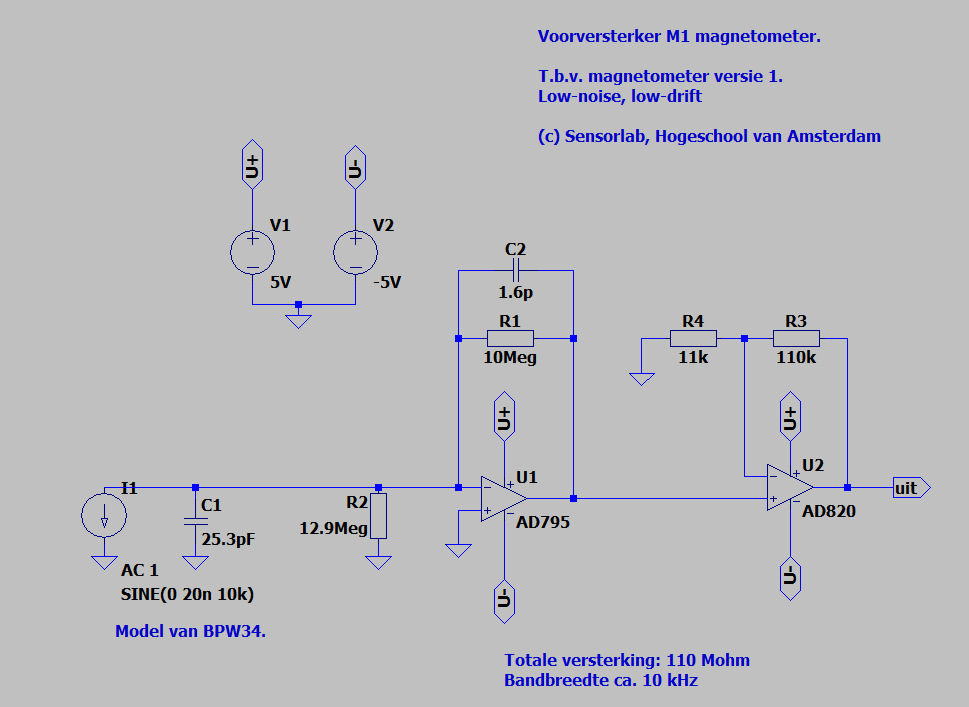
\includegraphics[width=0.7\linewidth]{img/photodetec_og}
	\caption{Provided photodetector design}
	\label{fig:photodetecog}
\end{figure}


\subsubsection{Simulation}
Tina-TI was used to simulate and visualize the DC gain and frequency response of the system, as seen in Figure \ref{fig:tina2probes}. The signals $V_{ot}$ and $V_{out}$ correspond to the output of the transimpedance and non-inverting amplification stage respectively. The AC plot (Figure \ref{fig:tinaac2probes}) shows the cutoff, at \num{10,77} \unit{\kilo \hertz}, and the gain inside the gain bandwidth, which is \num{160,82} \unit{\decibel}. The DC plot (Figure \ref{fig:tinadc2probes}) shows the voltage with respect to the current and demonstrates the linearity of the system in the range of \numrange{0}{46,31} \unit{\nano \ampere}. After $V_{out}$ reaches \num{5} \unit{V}, the output remains fixed, because it cannot exceed the voltage provided to the amplifier. 

\begin{figure}[ht]
	\centering
	\begin{subfigure}[1a]{.49\linewidth}
		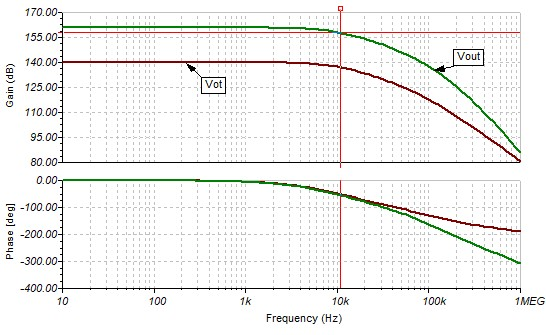
\includegraphics[width=\linewidth]{img/tina_AC_2probes}
		\caption{Frequency response}
		\label{fig:tinaac2probes}
	\end{subfigure}
	\hfill
	\begin{subfigure}[1b]{.49\linewidth}
		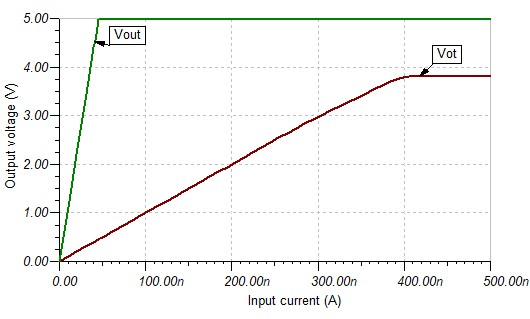
\includegraphics[width=\linewidth]{img/tina_DC_2probes}
		\caption{DC gain}
		\label{fig:tinadc2probes}
	\end{subfigure}
	\caption{Simulation of the first iteration of the photodetector}
	\label{fig:tina2probes}
\end{figure}


\subsubsection{Implementation} 
Figure \ref{fig:photodetecogpcb} shows the back side of the PCB. It hosts all components, except for the photodiode, which sits unobstructed on the front side. Requirements for the physical dimensions were also set by the client. The PCB needs to fit the Thorlabs mount standard, since the rest of the setup also uses it. 

\begin{figure}[ht]
	\centering
	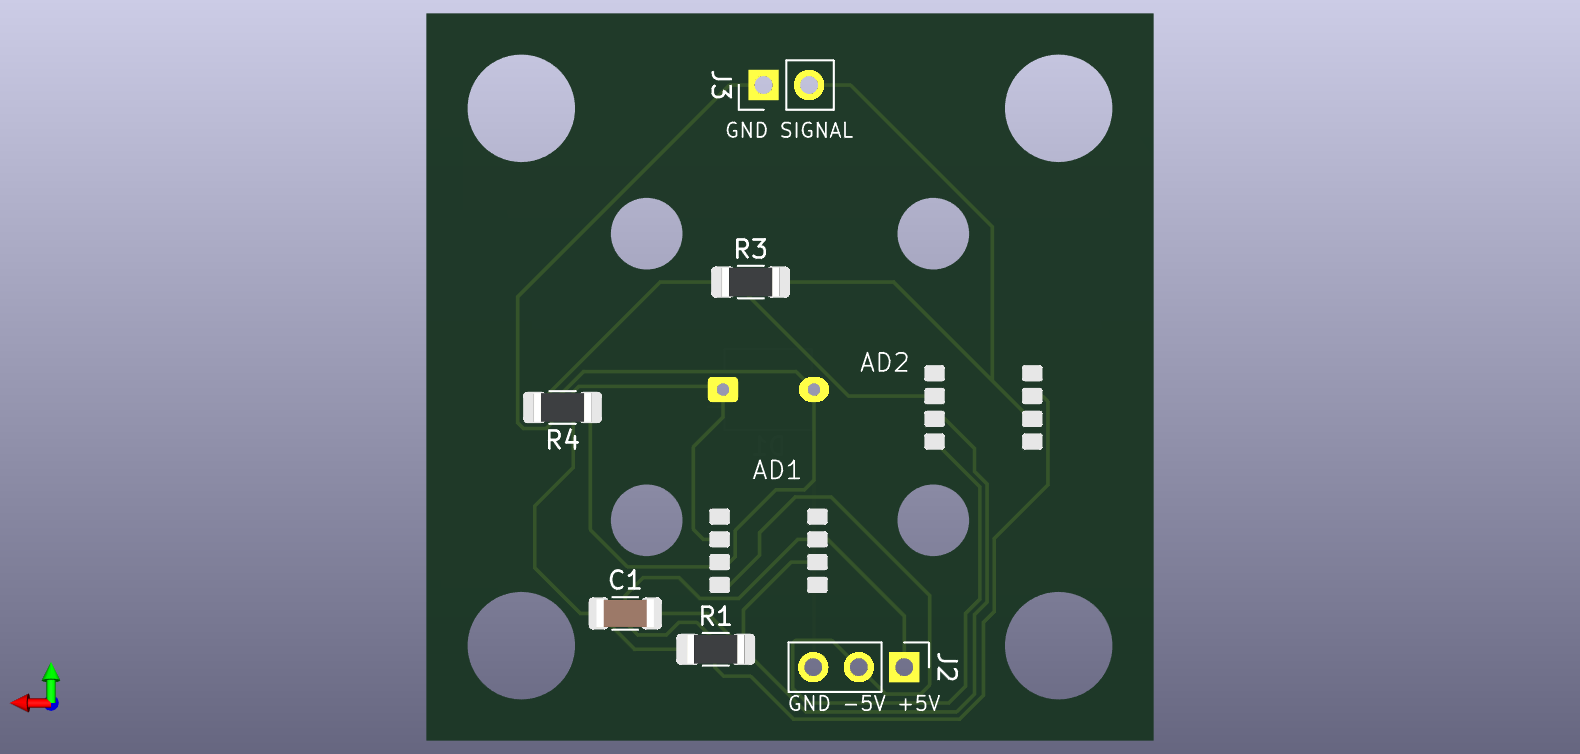
\includegraphics[width=0.7\linewidth]{img/photodetec_og_pcb}
	\caption{First iteration of the photodetection PCB}
	\label{fig:photodetecogpcb}
\end{figure}


\section{OLIA implementation}
